% Koko
\documentclass[blue,normal,cn]{elegantnote}
\usepackage{array}
\usepackage{courier}
\usepackage{xcolor}
\usepackage{zhnumber}
\usepackage{ulem}
\usepackage{float}

\definecolor{light-gray}{gray}{0.95}
\newcommand{\code}[1]{\colorbox{light-gray}{\texttt{#1}}}
\newfontfamily\courier{Courier New}
\lstset{linewidth=1.1\textwidth,
	numbers=left,
	basicstyle=\small\courier,
	numberstyle=\tiny\courier,
	keywordstyle=\color{blue}\courier,
	commentstyle=\it\color[cmyk]{1,0,1,0}\courier, 
	stringstyle=\it\color[RGB]{128,0,0}\courier,
	frame=single,
	backgroundcolor=\color[RGB]{245,245,244},
	breaklines,
	extendedchars=false, 
	xleftmargin=2em,xrightmargin=2em, aboveskip=1em,
	tabsize=4, 
	showspaces=false
	basicstyle=\small\courier
}
\title{实验 3: 使用 MIPS 指令实现求两个数组的点积}
\version{$\aleph$}
\date{\zhtoday}

\begin{document}
\author{
    \begin{tabular}[t]{c}
        于海鑫 \\
        2017211240
    \end{tabular}
}
\maketitle

\section{实验目的}
\begin{enumerate}
    \item 通过实验熟悉实验 1 和实验 2 的内容
    \item 增强汇编语言编程能力
    \item 学会使用模拟器中的定向功能进行优化
    \item 了解对代码进行优化的方法
\end{enumerate}

\section{实验平台}

实验平台采用指令级和流水线操作级模拟器 \code{MIPSsim}。

\section{实验内容和步骤}

\begin{enumerate}[wide=0pt, listparindent=2em, parsep=0pt]
    \item 自行编写一个计算两个向量点积的汇编程序,该程序要求可以实现求两个向量点积计算后的结果。

          向量的点积:假设有两个 n 维向量 a、b,则 a 与 b 的点积为:

          $$\vec{a}\cdot\vec{b} = \sum_{i=1}^{n} a_i b_i = a_1b_1 + \cdots + a_nb_n$$

          两个向量元素使用数组进行数据存储,\textbf{要求向量的维度不得小于 10}

    \item 启动 MIPSsim。
    \item 载入自己编写的程序,观察流水线输出结果。
    \item 使用定向功能再次执行代码,与刚才执行结果进行比较,观察执行效率的不同。
    \item 采用静态调度方法重排指令序列,减少相关,优化程序。
    \item 对优化后的程序使用定向功能执行,与刚才执行结果进行比较,观察执行效率的不同。
\end{enumerate}

\section{向量点积}

\subsection{代码}
向量点积程序使用 C 程序描述是很简单的,代码如下:

\begin{lstlisting}[language=C]
int naive_prod(int *a, int *b, int *n) {
    int size = *n;
    int result = 0;
    for(int i = 0; i < size; i++) {
        result += a[i] * b[i];
    }
    return result;
}
\end{lstlisting}

我们要做的仅仅就是把这段代码翻译成 MIPS 汇编即可,结果如下(需要注意 MIPS 的\href{https://courses.cs.washington.edu/courses/cse410/09sp/examples/MIPSCallingConventionsSummary.pdf}{\textbf{调用约定}})

\lstinputlisting{naive_prod.s}

\subsection{运行结果}

\subsubsection{未开启定向功能时}

\begin{lstlisting}
  汇总:
    执行周期总数:178
    ID段执行了98条指令

  硬件配置:
    内存容量:4096 B
    加法器个数:1		执行时间(周期数):6
    乘法器个数:1		执行时间(周期数)7		
    除法器个数:1		执行时间(周期数)10		
    定向机制:不采用

  停顿(周期数):
    RAW停顿:66		占周期总数的百分比:37.07865%
    其中:
      load停顿:22		占所有RAW停顿的百分比:33.33333%
      浮点停顿:0		占所有RAW停顿的百分比:0%
    WAW停顿:0		占周期总数的百分比:0%
    结构停顿:0		占周期总数的百分比:0%
    控制停顿:13		占周期总数的百分比:7.303371%
    自陷停顿:0		占周期总数的百分比:0%
    停顿周期总数:79	占周期总数的百分比:44.38202%

  分支指令:
    指令条数:12		占指令总数的百分比:12.2449%
    其中:
      分支成功:12		占分支指令数的百分比:100%
      分支失败:1		占分支指令数的百分比:8.333333%

  load/store指令:
    指令条数:24		占指令总数的百分比:24.4898%
    其中:
      load:24		占load/store指令数的百分比:100%
      store:0		占load/store指令数的百分比:0%

  浮点指令:
    指令条数:0		占指令总数的百分比:0%
    其中:
      加法:0		占浮点指令数的百分比:0%
      乘法:0		占浮点指令数的百分比:0%
      除法:0		占浮点指令数的百分比:0%

  自陷指令:
    指令条数:1		占指令总数的百分比:1.020408%
\end{lstlisting}

时钟周期图如下:

\begin{figure}[H]
    \centering
    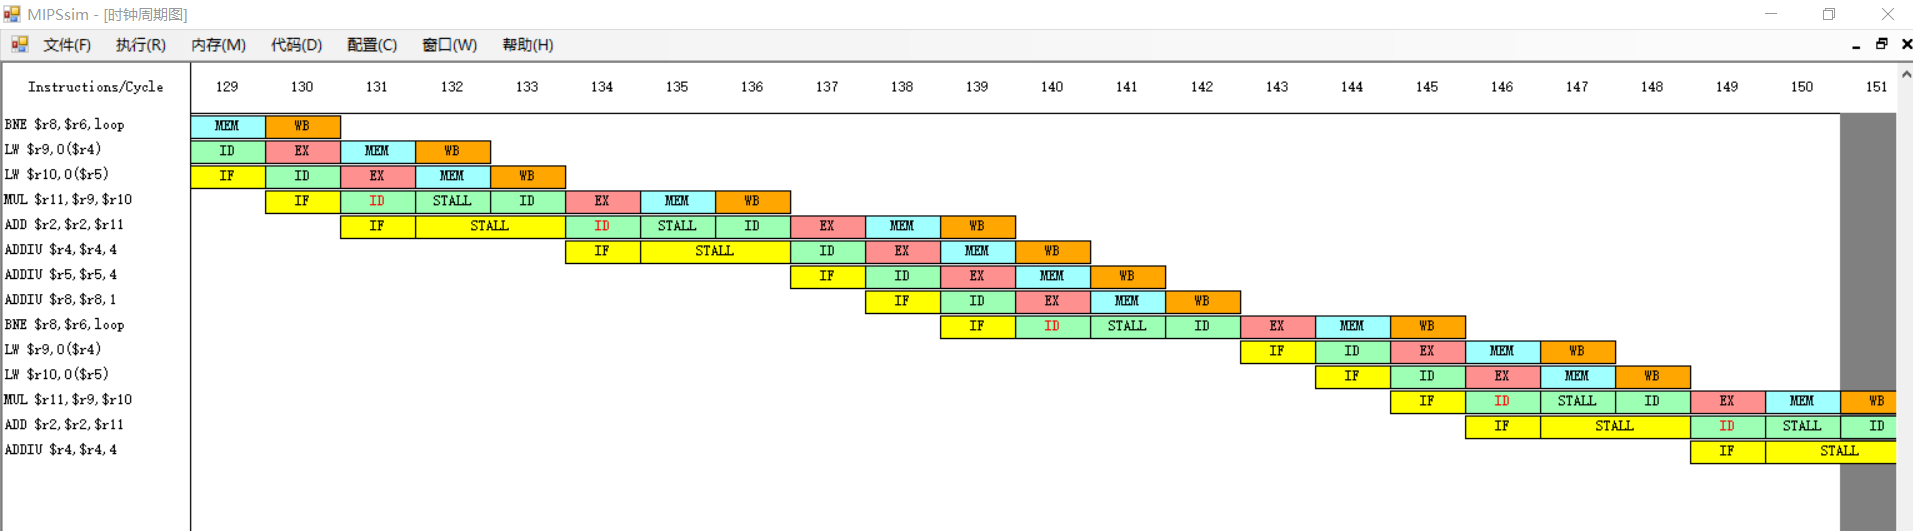
\includegraphics[width=.8\textwidth]{fig/naive_prod.png}
    \caption{时钟周期图}
    \label{fig:naive_prod}
\end{figure}

\subsubsection{开启定向功能后}

\begin{lstlisting}
  汇总:
    执行周期总数:134
    ID段执行了98条指令

  硬件配置:
    内存容量:4096 B
    加法器个数:1		执行时间(周期数):6
    乘法器个数:1		执行时间(周期数)7		
    除法器个数:1		执行时间(周期数)10		
    定向机制:采用

  停顿(周期数):
    RAW停顿:22		占周期总数的百分比:16.41791%
    其中:
      load停顿:11		占所有RAW停顿的百分比:50%
      浮点停顿:0		占所有RAW停顿的百分比:0%
    WAW停顿:0		占周期总数的百分比:0%
    结构停顿:0		占周期总数的百分比:0%
    控制停顿:13		占周期总数的百分比:9.701492%
    自陷停顿:0		占周期总数的百分比:0%
    停顿周期总数:35	占周期总数的百分比:26.1194%

  分支指令:
    指令条数:12		占指令总数的百分比:12.2449%
    其中:
      分支成功:12		占分支指令数的百分比:100%
      分支失败:1		占分支指令数的百分比:8.333333%

  load/store指令:
    指令条数:24		占指令总数的百分比:24.4898%
    其中:
      load:24		占load/store指令数的百分比:100%
      store:0		占load/store指令数的百分比:0%

  浮点指令:
    指令条数:0		占指令总数的百分比:0%
    其中:
      加法:0		占浮点指令数的百分比:0%
      乘法:0		占浮点指令数的百分比:0%
      除法:0		占浮点指令数的百分比:0%

  自陷指令:
    指令条数:1		占指令总数的百分比:1.020408%
\end{lstlisting}

时钟周期图如下:

\begin{figure}[H]
    \centering
    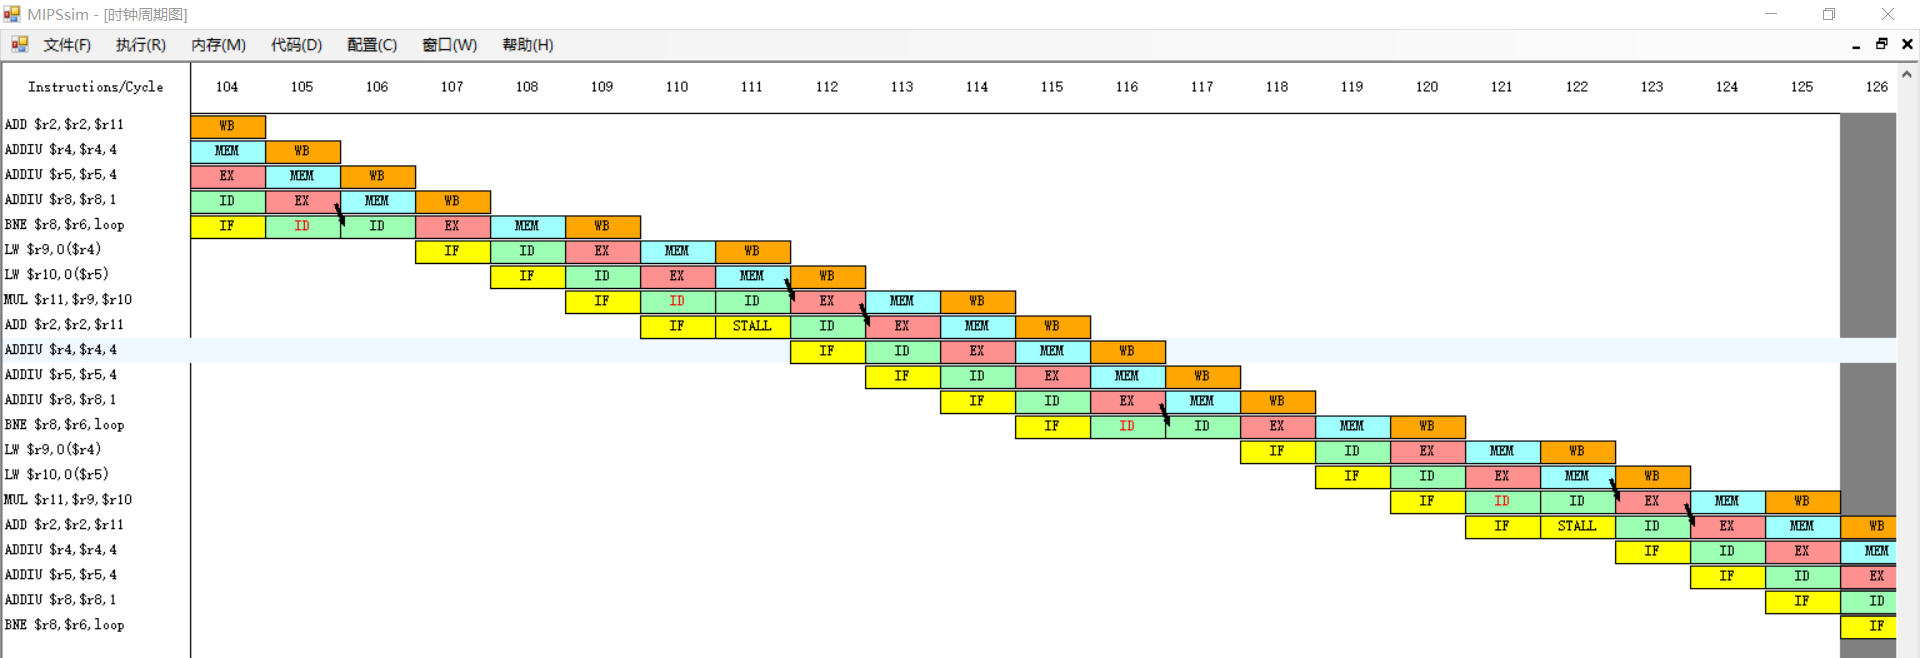
\includegraphics[width=.8\textwidth]{fig/naive_prod_bypass.png}
    \caption{时钟周期图}
    \label{fig:naive_prod_bypass}
\end{figure}

\section{优化后的向量点积}

\subsection{代码}

通过发现原始代码中的数据相关并将之规避掉,我们得到了如下的代码:

\lstinputlisting{prod.s}

\subsection{运行结果}

\begin{lstlisting}
  汇总:
    执行周期总数:112
    ID段执行了98条指令

  硬件配置:
    内存容量:4096 B
    加法器个数:1		执行时间(周期数):6
    乘法器个数:1		执行时间(周期数)7		
    除法器个数:1		执行时间(周期数)10		
    定向机制:采用

  停顿(周期数):
    RAW停顿:0		占周期总数的百分比:0%
    其中:
      load停顿:0		占所有RAW停顿的百分比:0%
      浮点停顿:0		占所有RAW停顿的百分比:0%
    WAW停顿:0		占周期总数的百分比:0%
    结构停顿:0		占周期总数的百分比:0%
    控制停顿:13		占周期总数的百分比:11.60714%
    自陷停顿:0		占周期总数的百分比:0%
    停顿周期总数:13	占周期总数的百分比:11.60714%

  分支指令:
    指令条数:12		占指令总数的百分比:12.2449%
    其中:
      分支成功:12		占分支指令数的百分比:100%
      分支失败:1		占分支指令数的百分比:8.333333%

  load/store指令:
    指令条数:24		占指令总数的百分比:24.4898%
    其中:
      load:24		占load/store指令数的百分比:100%
      store:0		占load/store指令数的百分比:0%

  浮点指令:
    指令条数:0		占指令总数的百分比:0%
    其中:
      加法:0		占浮点指令数的百分比:0%
      乘法:0		占浮点指令数的百分比:0%
      除法:0		占浮点指令数的百分比:0%

  自陷指令:
    指令条数:1		占指令总数的百分比:1.020408%
\end{lstlisting}

时钟周期图如下:

\begin{figure}[H]
    \centering
    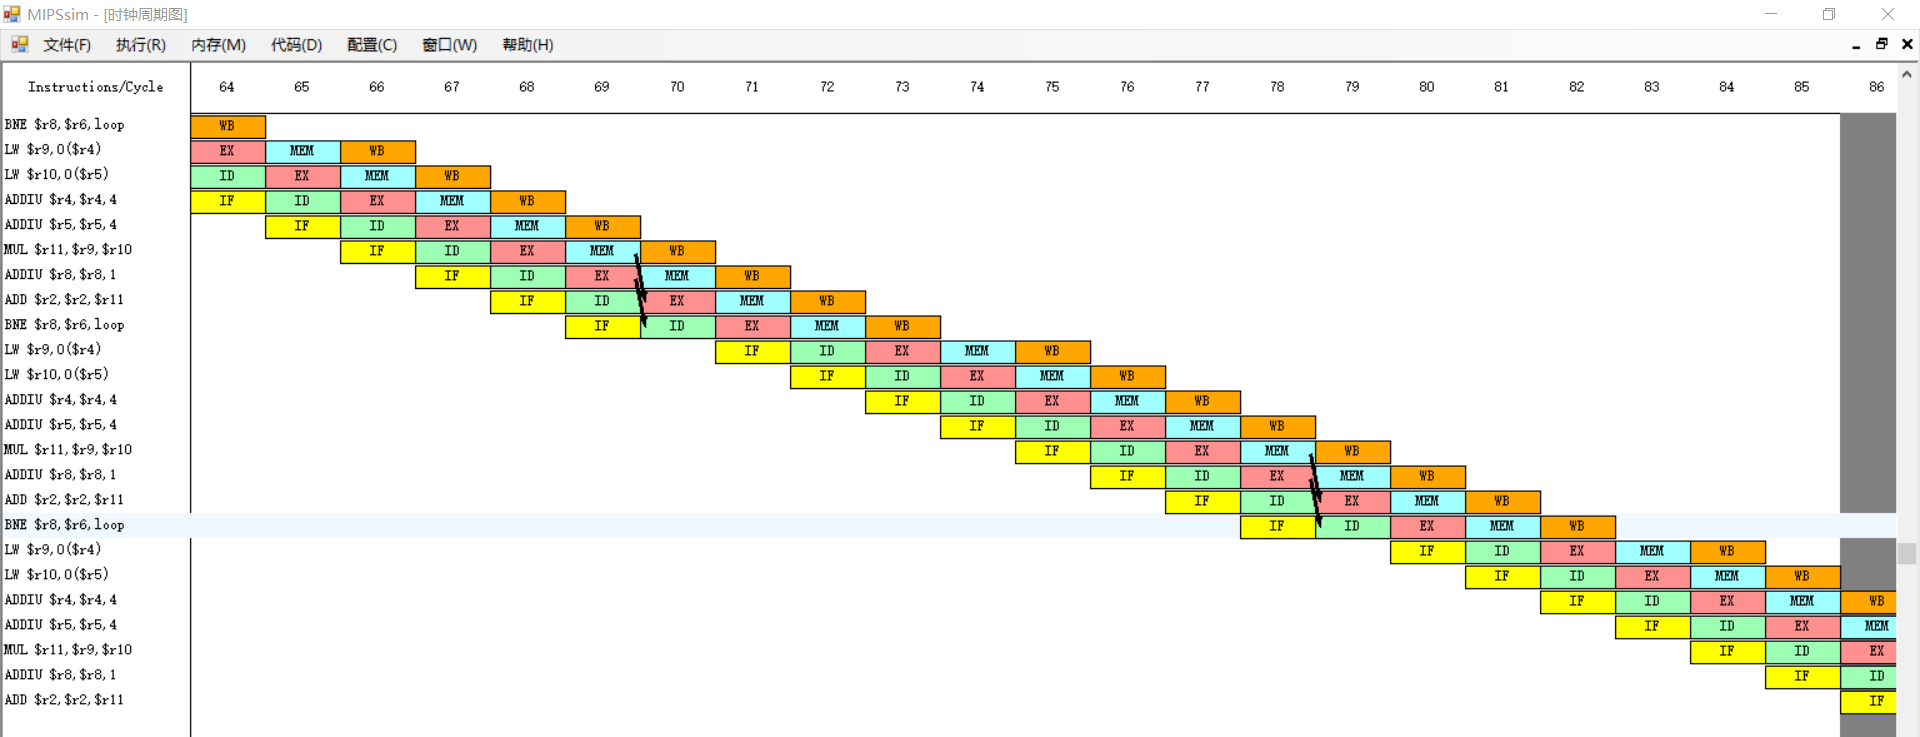
\includegraphics[width=.8\textwidth]{fig/prod_bypass.png}
    \caption{时钟周期图}
    \label{fig:prod_bypass}
\end{figure}

与之前的代码相比,效率大约是之前的 $134 / 112 = 1.19$ 倍。

\section{实验中的问题与心得}

本次实验主要是人肉模拟编译器做一些简单的优化,本次实验中遇到的问题有一部分指令没有在现有的 \code{MIPSsim} 模拟器上实现,比如实际编译器经常产生的 \code{BAL} 指令,推测是模拟器实现者水平有限,不过这类问题可以通过更换别的指令替代来解决,不是很影响实现。

本次的心得大约是通过一些静态优化,我们也可以很好的进一步榨取 CPU 的性能。

\end{document}